% \begin{chapter}*{}
%% Based on EN-Revision r229

% \aosafigure{../images/backmatter/making.pdf}{}{fig.making.making}
\thispagestyle{empty}

\sffamily

%% \Large You May Also Enjoy\ldots
\Large これもきっと気に入ると思うんだ\ldots

\normalsize

\begin{figure}[h!]
\centering
%% 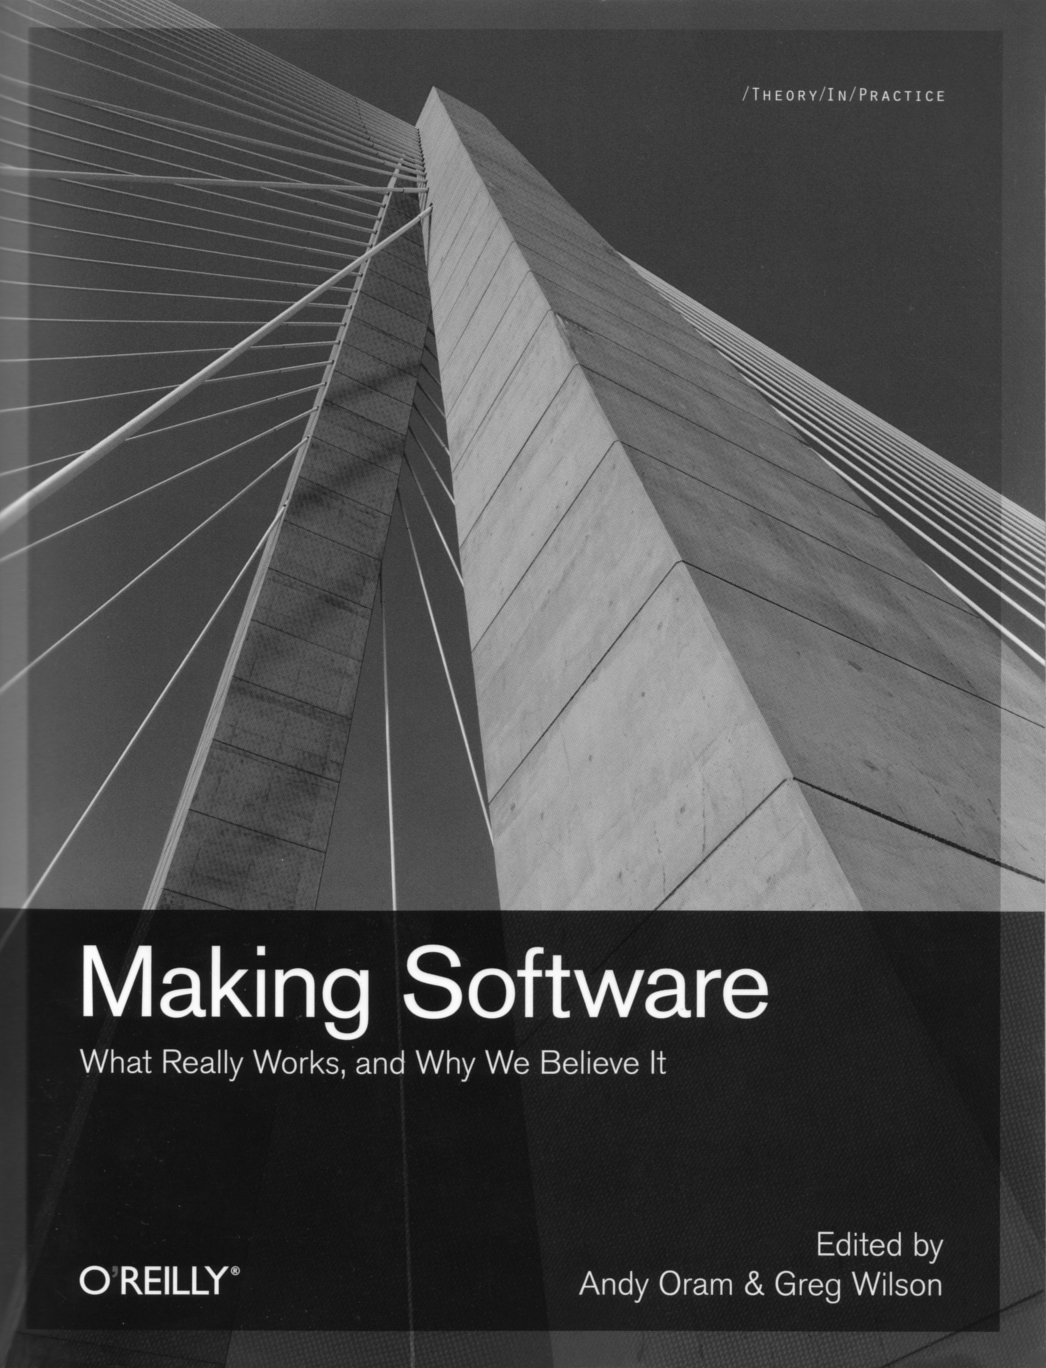
\includegraphics[width=250pt]{../images/backmatter/making.pdf}
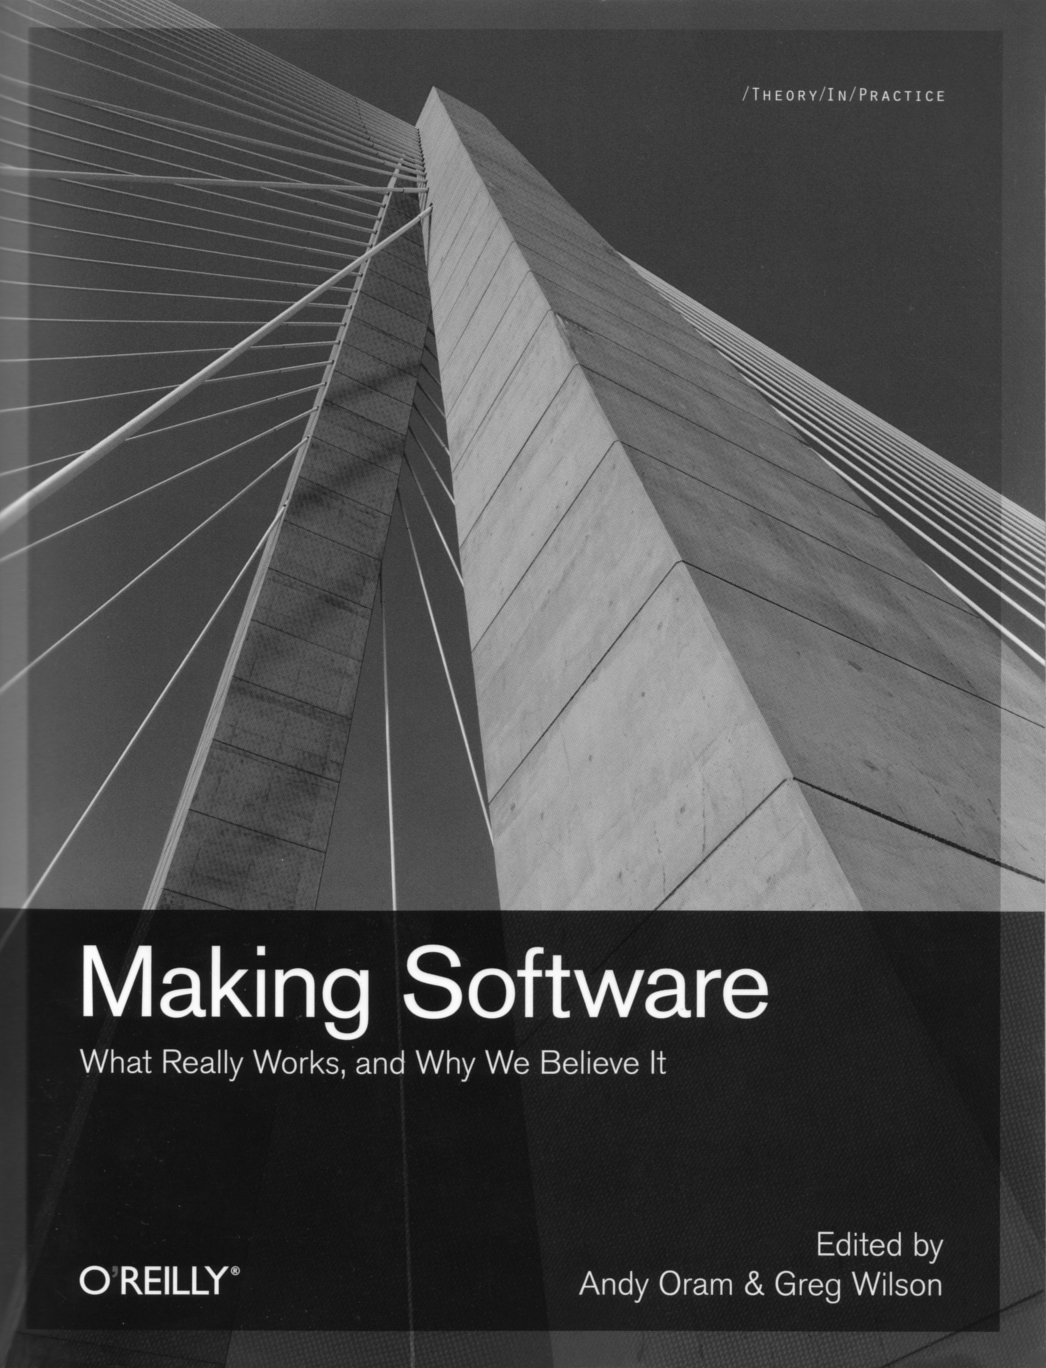
\includegraphics[width=250pt]{../images/backmatter/making.eps}
\end{figure}

%% Many claims are made about how certain tools, technologies, and
%% practices improve software development. But which are true, and which
%% are merely wishful thinking? In \emph{Making Software}, leading
%% researchers and practitioners present chapter-length summaries of key
%% empirical findings in software engineering, and answer questions like:
「このツールを使えばソフトウェア開発がより改善できるよ!」「このテクノロジーを使えば…!」「このプラクティスを使えば…!」…こんな主張があふれかえっている。しかし、その中で真実はどれくらいあるだろうか?中には、単なる希望的観測に過ぎないものもあるんじゃないかな?\emph{Making Software}は、トップレベルの研究者や実務者たちが、ソフトウェア開発の世界での実証に基づくさまざまな発見をまとめたものだ。こんな疑問に対する答えが書かれている。

\vspace{-0.1cm}

\begin{aosaitemize}

%% \item Are some programmers really ten times more productive than others?
\item 優秀なプログラマーは凡人の10倍の生産性がある?

%% \item Does writing tests first help you develop better code faster?
\item テストファーストを採用すれば、よりよいコードをより高速に書けるようになる?

%% \item Can code metrics predict the number of bugs in a piece of software?
\item コードメトリクスで、ソフトウェアのバグの数を予想できる?

%% \item Does using design patterns actually make software better?
\item デザインパターンって、実際のところどうなの?

%% \item What effect does personality have on pair programming?
\item ペアプログラミングって、どんな効果がある?

%% \item What matters more: how far apart people are geographically, or how far apart they are in the org chart?
\item 地理的に離れていることと、組織体系上で離れていること。どちらのほうが影響が大きい?

\end{aosaitemize}

\vspace{-0.2cm}

\setlength{\parskip}{0.15cm}

%% \noindent As with \emph{The Architecture of Open Source Applications}, royalties
%% from \emph{Making Software} will be donated to Amnesty International.
\noindent \emph{The Architecture of Open Source Applications}と同様、\emph{Making Software}の収益もアムネスティ・インターナショナルに寄付される。

%% \noindent \emph{Making Software: What Really Works, and Why We Believe It} \\
%% edited by Andy Oram and Greg Wilson \\
%% O'Reilly Media, 2010, 978-0596808327 \\
%% \url{http://oreilly.com/catalog/9780596808303}
\noindent \emph{Making Software: What Really Works, and Why We Believe It} \\
edited by Andy Oram and Greg Wilson \\
O'Reilly Media, 2010, 978-0596808327 \\
\url{http://oreilly.com/catalog/9780596808303}

\normalfont

\pagebreak
\thispagestyle{empty}

